\documentclass[conference]{IEEEtran}

\usepackage[utf8]{inputenc}
\usepackage[T1]{fontenc}
\usepackage{amsmath,amssymb}
\usepackage{booktabs}
\usepackage{tabularx}
\usepackage{array}
\usepackage{xcolor}
\usepackage{tikz}
\usetikzlibrary{arrows.meta,positioning,fit,backgrounds,calc}
\usepackage[hidelinks]{hyperref}

\newcommand{\tauext}{\tau_{\mathrm{ext}}}

% Let wide figures and tables share pages with text instead of floating to
% their own pages.
\renewcommand{\topfraction}{0.9}
\renewcommand{\dbltopfraction}{0.9}
\renewcommand{\textfraction}{0.07}
\renewcommand{\floatpagefraction}{0.8}
\renewcommand{\dblfloatpagefraction}{0.8}
\setcounter{topnumber}{3}
\setcounter{dbltopnumber}{2}
% Stack floats from the top of float-only pages instead of spreading them out.
\makeatletter
\setlength{\@dblfptop}{0pt}
\setlength{\@dblfpsep}{14pt plus 2pt}
\setlength{\@dblfpbot}{0pt plus 1fil}
\setlength{\@fptop}{0pt}
\setlength{\@fpsep}{14pt plus 2pt}
\setlength{\@fpbot}{0pt plus 1fil}
\makeatother
\newcolumntype{L}{>{\raggedright\arraybackslash}X}

\begin{document}

\title{Blind Proprioceptive Localization and\\Peg Insertion on a Franka Arm}

\author{\IEEEauthorblockN{Team Kilo}
\IEEEauthorblockA{16-662 Robot Autonomy, Fall 2026\\
Project proposal}}

\maketitle

\begin{abstract}
We propose a Franka arm that picks up a peg from a known holder, finds a
taped-down box by touching it with the peg, and inserts the peg into the box's
hole, using only its own joint sensing: no camera, no wrist force-torque
sensor, and no prior knowledge of where the box or hole is. Phase~1 localizes
the box with sideways approach-until-contact probes made with the side of the
peg's shaft and a particle filter, then searches the region around the box
centre for the hole. Phase~2 inserts the peg with a reinforcement-learning policy trained
in MuJoCo, which reads a short history of joint states and the Franka's
estimated external joint torques. The estimation error measured in Phase~1 sets
the hole-position noise Phase~2 is trained against. We will evaluate
localization accuracy, insertion success against a scripted spiral baseline, the
value of torque sensing, and a full end-to-end run on the real robot.
\end{abstract}

\section{Introduction}

Vision struggles exactly where assembly gets hard: the held part blocks the
camera's view of the hole, and millimetre clearances are below what a camera
reliably resolves. The course setup also provides no cameras. A robot's own
joint sensing, by contrast, is always available and sits right at the contact.

Bronars, Park \emph{et al.}~\cite{bronars2026blind} show that a policy using
only joint positions, velocities and previous actions can insert pegs, mesh
gears and thread nuts. It is trained with PPO~\cite{schulman2017ppo} entirely
in simulation and transfers zero-shot to a real arm for peg insertion. It
deliberately uses no force or torque sensing, and each episode starts with the
part already touching the fixture near the hole. Their companion tool
mjfit~\cite{mjfit} generates exact convex MuJoCo~\cite{todorov2012mujoco}
collision geometry for pegs and holes; we use it to build our simulated box and
hole.

We extend this setting in three ways:
\begin{itemize}
  \item \textbf{Finding the hole first.} Phase~1 removes the assumption that the
  part starts near the hole by locating the box and hole by touch.
  \item \textbf{Torque sensing.} The Franka reports estimated external joint
  torques $\tauext$. We test whether adding them helps over joint positions and
  velocities alone.
  \item \textbf{Estimation-aware training.} Phase~2 is trained against the error
  Phase~1 actually achieves on the real robot, not a guessed range.
\end{itemize}

\section{Problem Statement and Assumptions}

\textbf{Given} a peg at a fixed, known location and a box with one vertical hole
at an unknown position on the table, \textbf{grasp} the peg, \textbf{find} the
hole and \textbf{insert} the peg, using only joint positions $q$, velocities
$\dot q$ and estimated external torques $\tauext$.

\begin{itemize}
  \item \textbf{Peg design:} a square top, so the gripper always holds it the
  same way, and a 25\,mm diameter round shaft with a 1\,mm chamfer at the tip.
  Because the shaft is round, the peg's rotation does not matter for insertion.
  \item \textbf{Peg pickup:} pegs sit in a holder at a fixed, known pose, so they
  are never localized. The robot grasps one and keeps it for the whole run.
  \item \textbf{Peg as probe:} the box is found with the side of the
  cylindrical shaft, held vertical. A contact anywhere on it puts the box wall
  exactly one shaft radius (12.5\,mm) from the peg's axis, whatever the wrist
  angle. The gripper fingers are not rotationally symmetric, so they are never
  used to probe.
  \item \textbf{Box:} 3D-printed, $126.7\times169\times50.8$\,mm, taped to the table
  at an unknown position and rotation inside a region of about
  $30\times30$\,cm in the clear table area in front of the robot.
  \item \textbf{Hole:} one vertical 25.4\,mm through-hole with a 1\,mm chamfer
  at the top edge, never angled, within a known radius $R$ of the box's top-face
  centre but not necessarily at it (4\,mm off-centre in the current CAD). $R$ is
  still to be set.
  \item \textbf{Clearance:} 0.4\,mm diametral (25.4\,mm hole, 25.0\,mm shaft),
  before printing error. A looser base of about 1.5\,mm may be printed to stage
  the difficulty.
  \item \textbf{Control:} Cartesian impedance control at low stiffness, about
  1--2\,cm/s while probing, with the Franka's collision thresholds raised so
  contact does not trigger its safety stop.
\end{itemize}

\textbf{Out of scope:} finding the pegs, boxes that move, angled holes, threads
and gears.

\section{System Architecture}

Fig.~\ref{fig:arch} shows the system. Both phases send motion targets to the
same impedance controller and read the same joint signals; only Phase~2's policy
is learned. Phase~1's measured error sets the hole-position noise used in
simulation training, so the deployed policy is trained for the estimates it
will actually receive.

\begin{figure*}[t]
\centering
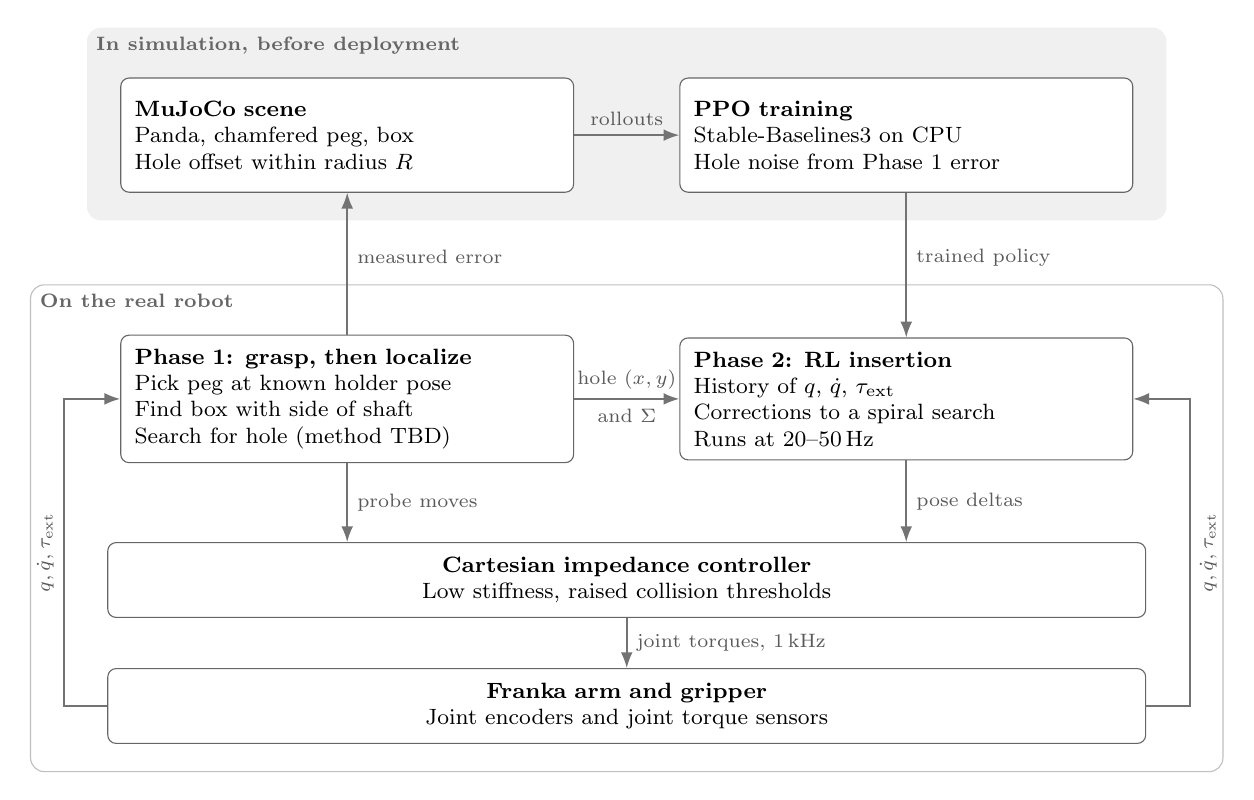
\begin{tikzpicture}[
  font=\footnotesize,
  box/.style={draw=black!60, rounded corners=3pt, align=left, inner sep=5pt,
              text width=5.4cm, minimum height=1.45cm, fill=white},
  wide/.style={draw=black!60, rounded corners=3pt, align=center, inner sep=4pt,
               text width=12.9cm, minimum height=0.95cm, fill=white},
  arr/.style={-{Latex[length=2mm]}, draw=black!55, line width=0.6pt},
  lbl/.style={font=\scriptsize, text=black!65},
  zone/.style={rounded corners=5pt, inner xsep=12pt, inner ysep=10pt},
]
  \node[box] (mj)  at (-3.55, 0)    {\textbf{MuJoCo scene}\\Panda, chamfered peg, box\\Hole offset within radius $R$};
  \node[box] (ppo) at ( 3.55, 0)    {\textbf{PPO training}\\Stable-Baselines3 on CPU\\Hole noise from Phase~1 error};
  \node[box] (p1)  at (-3.55,-3.35) {\textbf{Phase 1: grasp, then localize}\\Pick peg at known holder pose\\Find box with side of shaft\\Search for hole (method TBD)};
  \node[box] (p2)  at ( 3.55,-3.35) {\textbf{Phase 2: RL insertion}\\History of $q$, $\dot q$, $\tauext$\\Corrections to a spiral search\\Runs at 20--50\,Hz};
  \node[wide] (ctrl) at (0,-5.65)   {\textbf{Cartesian impedance controller}\\Low stiffness, raised collision thresholds};
  \node[wide] (fr)   at (0,-7.25)   {\textbf{Franka arm and gripper}\\Joint encoders and joint torque sensors};

  \coordinate (lw) at (-7.15,-7.25);
  \coordinate (rw) at ( 7.15,-7.25);

  \begin{scope}[on background layer]
    \node[zone, fill=black!6, fit=(mj)(ppo), yshift=4pt, inner ysep=14pt] (zs) {};
    \node[anchor=north west, font=\scriptsize\bfseries, text=black!60] at (zs.north west) {In simulation, before deployment};
    \node[zone, draw=black!25, fit=(p1)(p2)(fr)(lw)(rw), yshift=4pt, inner ysep=14pt] (zr) {};
    \node[anchor=north west, font=\scriptsize\bfseries, text=black!60] at (zr.north west) {On the real robot};
  \end{scope}

  \draw[arr] (mj) -- node[lbl, above] {rollouts} (ppo);
  \draw[arr] (ppo.south) -- node[lbl, right, pos=0.45] {trained policy} (p2.north);
  \draw[arr] (p1.north) -- node[lbl, right, pos=0.55] {measured error} (mj.south);
  \draw[arr] (p1) -- node[lbl, above] {hole $(x,y)$} node[lbl, below] {and $\Sigma$} (p2);
  \draw[arr] (p1.south) -- node[lbl, right] {probe moves} (p1.south |- ctrl.north);
  \draw[arr] (p2.south) -- node[lbl, right] {pose deltas} (p2.south |- ctrl.north);
  \draw[arr] (ctrl) -- node[lbl, right] {joint torques, 1\,kHz} (fr);
  \draw[arr] (fr.west) -- (lw) |- node[lbl, sloped, above, pos=0.25] {$q,\dot q,\tauext$} (p1.west);
  \draw[arr] (fr.east) -- (rw) |- node[lbl, sloped, below, pos=0.25] {$q,\dot q,\tauext$} (p2.east);
\end{tikzpicture}
\caption{System architecture. A policy trained in simulation is deployed as
Phase~2; Phase~1's measured localization error feeds back into training.}
\label{fig:arch}
\end{figure*}

\section{Phase 1: Grasping the Peg, then Finding the Box and Hole}

Phase~1 outputs the hole centre $(x,y)$ with covariance $\Sigma$, plus the box's
top-surface height. Because the hole is vertical and the shaft round, no
orientation is estimated.

\textbf{Basic move: approach until contact.} Move along a direction at low speed
until $\tauext$ (or the Franka's Cartesian contact flags) crosses a calibrated
threshold, and record the peg's position by forward kinematics. For a sideways
move the wall lies one shaft radius from the peg's axis along the direction of
travel, so each contact gives one wall point; each move that ends without contact
is also evidence that nothing lies along that path.

\begin{enumerate}
  \item \textbf{Grasp the peg} at the holder's known pose. The square top seats
  the peg the same way every time, so its axis and length relative to the
  gripper are calibrated once.
  \item \textbf{Table height} from one downward touch.
  \item \textbf{Coarse search:} sideways sweeps across the region with the peg
  vertical and the lower shaft below the box's top, until the side of the
  shaft hits a wall.
  \item \textbf{Box pose:} a particle filter~\cite{thrun2005probabilistic} over
  the box centre and rotation. Each wall point is scored by its distance to the
  box's known outline; free sweeps remove particles whose box would overlap the
  swept shaft. The next probe goes to the side whose predicted contact varies
  most across particles, and probing stops when the centre is known to about
  2\,mm. One downward touch on the top face gives its height.
  \item \textbf{Hole search (strategy to be decided):} start from the box-centre
  estimate, with the hole somewhere in a disc of radius $R$ around it, widened by
  the centre's uncertainty. Whatever the sensing, a particle filter over the
  hole's $(x,y)$ can fuse the measurements and choose the next one.
  \item \textbf{Hand off:} once the hole is found, the arm lifts the peg to a
  known hover pose above the estimate for Phase~2.
\end{enumerate}

Ground truth for evaluation comes from guiding the arm by hand until the peg is
seated, then reading its pose by forward kinematics. A stretch goal replaces the
hand-written probe rule with an information-gain or RL probing policy.

\begin{table*}[t]
\caption{Planned experiments}
\label{tab:exp}
\centering
\footnotesize
\begin{tabularx}{\textwidth}{@{}>{\raggedright\arraybackslash}p{2.6cm}LLL>{\raggedright\arraybackslash}p{2.3cm}@{}}
\toprule
Experiment & Question & Conditions & Metrics & Trials \\
\midrule
E1: localization & How accurately can touch alone find the hole? & Random box placements and hole offsets within $R$ & Box- and hole-centre error (mm), number of contacts, time (s) & $\sim$20 real \\
E2: insertion in sim & Does RL beat the scripted spiral? & Spiral vs.\ spiral + RL vs.\ full RL & Success rate, time to insert, peak force, path length & 500+ simulated per condition \\
E3: torque ablation & Does $\tauext$ help over joint state alone? & RL with $q,\dot q$ vs.\ $q,\dot q,\tauext$ & Same as E2 & Simulated + $\sim$10 real each \\
E4: noise level & Does training on measured Phase~1 error matter? & Training noise at $1\times$ vs.\ $2\times$ measured error & Same as E2 & Simulated \\
E5: real insertion & Does the policy transfer to the real Franka? & Spiral vs.\ best RL policy, from Phase~1 estimates & Same as E2 & $\sim$20 real each \\
E6: end to end & Does the full system work? & Grasp peg $\rightarrow$ localize $\rightarrow$ insert, random box placement & Success per phase and overall, total time & 15--20 real \\
E7: clearance (stretch) & How much does clearance matter? & 0.4\,mm base vs.\ a looser (about 1.5\,mm) base & Success rate & $\sim$10 real \\
\bottomrule
\end{tabularx}
\end{table*}

\section{Phase 2: RL Insertion at the Found Hole}

Phase~2 trains a policy in simulation that inserts the peg from Phase~1's
estimate, correcting for its error by feel (Table~\ref{tab:phase2}). Until
Phase~1 has real error numbers, training uses a guessed range of $\pm5$\,mm. The
baseline is the same scripted spiral search without learned corrections.

\begin{table}[t]
\caption{Phase 2 design}
\label{tab:phase2}
\centering
\footnotesize
\begin{tabularx}{\columnwidth}{@{}>{\raggedright\arraybackslash}p{1.45cm}L@{}}
\toprule
Element & Design \\
\midrule
Simulator & MuJoCo with the Menagerie~\cite{menagerie2022} Franka Panda; 1\,ms timestep, as mjfit recommends \\
Peg model & From the team's CAD as two convex pieces: a box for the square top and a cylinder with a 1\,mm chamfer for the shaft \\
Box model & $126.7\times169\times50.8$\,mm block with a 25.4\,mm chamfered through-hole (0.4\,mm clearance), built with mjfit; hole offset from the box centre uniform within $R$ \\
Start state & Peg hovering above the estimated hole; true offset sampled from Phase~1's measured error, inflated about $1.5\times$; small grasp offset and tilt \\
Observation & 0.3--0.6\,s history of $q$, $\dot q$, $\tauext$, plus the estimated hole centre relative to the peg tip \\
Action & End-effector position deltas $(x,y,z)$ to Cartesian impedance control at 20--50\,Hz; no rotation \\
Policy form & Corrections added to a spiral search (main) or a full policy (comparison) \\
Reward & Dense peg-tip distance to hole bottom; insertion bonus; penalties for contact force and time \\
Training & PPO in Stable-Baselines3~\cite{raffin2021sb3} on CPU, vectorized environments \\
\bottomrule
\end{tabularx}
\end{table}

\section{Experiments and Metrics}

Table~\ref{tab:exp} lists the experiments. Real-robot trial counts are sized to
fit about six days of robot time on a robot shared with other groups. Success
rates are reported with 95\% confidence intervals, since trial counts are small.


\section{Timeline and Team Roles}

The two phases are built in parallel in the first week and merged on the real
robot in the second (Fig.~\ref{fig:timeline}), assuming work starts Monday,
Nov~23. Phase~1's measured error (day~7) becomes Phase~2's training noise. The
progress presentation (Nov~30 or Dec~2) falls after the first week, when
localization results and simulated insertion results should both be in hand.
Days after Dec~6 are buffer for the report and video, due Dec~11.

\begin{figure*}[t]
\centering
\def\dw{0.92}
\def\tlx{2.4}
\newcommand{\task}[5]{%
  \draw[#5, rounded corners=3pt] ({\tlx+(#1-1)*\dw+0.05},{#3-0.4}) rectangle ({\tlx+#2*\dw-0.05},{#3+0.4});
  \node[align=center, font=\scriptsize] at ({\tlx+(#1-1+#2)*\dw/2},#3) {#4};}
\begin{tikzpicture}
  \foreach \d [evaluate=\d as \dt using {int(\d<9 ? \d+22 : \d-8)}] in {1,...,14}
    \node[font=\scriptsize, text=black!60] at ({\tlx+(\d-0.5)*\dw},0.75) {\dt};
  \node[font=\scriptsize\bfseries, text=black!60] at ({\tlx+4*\dw},1.2) {Nov};
  \node[font=\scriptsize\bfseries, text=black!60] at ({\tlx+11.5*\dw},1.2) {Dec};
  \foreach \d in {1,8,15}
    \draw[black!20] ({\tlx+(\d-1)*\dw},1.35) -- ({\tlx+(\d-1)*\dw},-2.95);
  \draw[black!45, dashed] ({\tlx+7.5*\dw},0.5) -- ({\tlx+7.5*\dw},-1.85);
  \draw[black!45, dashed] ({\tlx+9.5*\dw},0.5) -- ({\tlx+9.5*\dw},-1.85);
  \node[font=\scriptsize, text=black!60, align=center] at ({\tlx+8.5*\dw},-0.1) {progress\\talk};

  \node[anchor=west, align=left, font=\footnotesize] at (0,0)    {\textbf{Phase 1}\\[-1pt]{\scriptsize real robot}};
  \node[anchor=west, align=left, font=\footnotesize] at (0,-1.2) {\textbf{Phase 2}\\[-1pt]{\scriptsize simulation}};
  \node[anchor=west, align=left, font=\footnotesize] at (0,-2.4) {\textbf{Whole team}\\[-1pt]{\scriptsize real robot}};

  \task{1}{2}{0}{Setup,\\peg grasp}{draw=black!60}
  \task{3}{5}{0}{Box\\localization}{draw=black!60}
  \task{6}{7}{0}{Hole\\search}{draw=black!60}
  \task{1}{2}{-1.2}{Sim\\scene}{draw=black!60}
  \task{3}{5}{-1.2}{Spiral +\\PPO env}{draw=black!60}
  \task{6}{7}{-1.2}{Train on\\real error}{draw=black!60}
  \task{8}{9}{-2.4}{Integrate\\phases}{draw=black!60}
  \task{10}{11}{-2.4}{Real\\insertion}{draw=black!60}
  \task{12}{14}{-2.4}{End to end,\\video, report}{draw=blue!60!black, fill=blue!8, line width=0.9pt}

  \draw[-{Latex[length=2mm]}, black!55] ({\tlx+6*\dw},-0.4) -- ({\tlx+6*\dw},-0.8)
    node[midway, right, font=\scriptsize, text=black!65] {error};
\end{tikzpicture}
\caption{Two-week schedule (days labelled by date). Both phases run in parallel
in week one, then merge on the robot.}
\label{fig:timeline}
\end{figure*}

\begin{table}[t]
\caption{Team roles}
\label{tab:roles}
\centering
\footnotesize
\begin{tabularx}{\columnwidth}{@{}>{\raggedright\arraybackslash}p{2.1cm}>{\raggedright\arraybackslash}p{0.9cm}L@{}}
\toprule
Role & People & Owns \\
\midrule
Phase 1 lead & 1--2 & Robot interface, contact detection, particle filters, E1 \\
Phase 2 lead & 1--2 & MuJoCo environment, spiral baseline, PPO, E2--E4 \\
Experiments and write-up & shared & Real trials E5--E7, plots, video, report \\
\bottomrule
\end{tabularx}
\end{table}

\section{Risks and Mitigations}

Table~\ref{tab:risks} lists the main risks. All robot runs follow the course
safety rules: never alone, and one person always on the emergency stop.

\begin{table*}[t]
\caption{Risks and mitigations}
\label{tab:risks}
\centering
\footnotesize
\begin{tabularx}{\textwidth}{@{}>{\raggedright\arraybackslash}p{4.4cm}>{\raggedright\arraybackslash}p{4.2cm}L@{}}
\toprule
Risk & Effect & Mitigation \\
\midrule
Printed hole comes out undersized & Peg does not fit at 0.4\,mm clearance & Print a short test ring of the hole first; adjust the CAD hole diameter to the measured print error \\
Peg slips or tilts in the gripper during probing & Peg axis offset changes, so every wall point is off & Square top seated against the fingers; high grip force; re-check against the table between phases \\
Tape lets the box shift under side probes & Box estimate drifts & Strong tape or clamps; low stiffness and speed; probe sides before the top \\
Phantom contacts in $\tauext$ from model error & False contact points corrupt the filter & Move slowly; calibrate thresholds on day 1; require the threshold to hold for several samples \\
Hole-search strategy not settled early & Phase~1 slips; Phase~2 lacks real error numbers & Choose the strategy by day 3; until then Phase~2 trains on the guessed $\pm5$\,mm range \\
Insertion jams (0.4\,mm clearance, flat end face) & Real insertions fail & Low rotational stiffness so the peg can self-align; start on a looser base if needed; the policy sees $\tauext$ and can learn to wiggle \\
Policy fails to transfer from simulation & No real RL result & Policy only corrects the spiral, so the spiral still works; report the gap; tune impedance gains to match simulation \\
Little robot time (robot shared by 2--3 groups) & Real trials cut short & Develop Phase~2 entirely in simulation; book robot slots in week one \\
\bottomrule
\end{tabularx}
\end{table*}

\section{Deliverables and Resources}

\textbf{Deliverables:} code (MuJoCo environment, Phase~1 localization, trained
policies, robot scripts); results for E1--E6, and E7 if time allows; a 1--3
minute video of the end-to-end run; the progress presentation; and a final
report in this format.

\textbf{Resources:} the course Franka arm with its gripper and control stack,
about six days of robot time; a 3D printer for the box, pegs and peg holder;
tape or clamps; and one multi-core workstation for simulation and PPO (a GPU is
optional).

\begin{thebibliography}{9}
\bibitem{bronars2026blind}
A.~Bronars, Y.~Park, K.~Kedia, and P.~Agrawal, ``Blind precise assembly:
Proprioceptive sim-to-real peg-in-hole for diverse parts,'' arXiv:2610.23849,
2026. [Online]. Available: \url{https://younghyopark.me/blind-proprioceptive-assembly/}

\bibitem{mjfit}
Y.~Park, ``mjfit: Exact convex collision geometry for MuJoCo,'' 2026.
[Online]. Available: \url{https://github.com/younghyopark/mjfit}

\bibitem{todorov2012mujoco}
E.~Todorov, T.~Erez, and Y.~Tassa, ``MuJoCo: A physics engine for model-based
control,'' in \emph{Proc. IEEE/RSJ IROS}, 2012, pp.~5026--5033.

\bibitem{menagerie2022}
K.~Zakka, Y.~Tassa, and MuJoCo Menagerie contributors, ``MuJoCo Menagerie: A
collection of high-quality simulation models for MuJoCo,'' 2022. [Online].
Available: \url{https://github.com/google-deepmind/mujoco_menagerie}

\bibitem{schulman2017ppo}
J.~Schulman, F.~Wolski, P.~Dhariwal, A.~Radford, and O.~Klimov, ``Proximal
policy optimization algorithms,'' arXiv:1707.06347, 2017.

\bibitem{raffin2021sb3}
A.~Raffin, A.~Hill, A.~Gleave, A.~Kanervisto, M.~Ernestus, and N.~Dormann,
``Stable-Baselines3: Reliable reinforcement learning implementations,''
\emph{J. Mach. Learn. Res.}, vol.~22, no.~268, pp.~1--8, 2021.

\bibitem{thrun2005probabilistic}
S.~Thrun, W.~Burgard, and D.~Fox, \emph{Probabilistic Robotics}. Cambridge, MA:
MIT Press, 2005.
\end{thebibliography}

\end{document}
